\part{Process and Thread Management}

\begin{figure}
  \center
  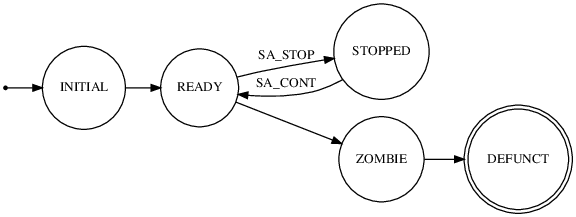
\includegraphics[width=10cm]{gfx/proc-states}
  \caption{Process states.}
  \label{figure:procstates}
\end{figure}

The process and thread management in Zeke is based on an idea that
a process is a container for threads owned by the process and it manages
the memory space used by its threads. Naturally this means that a process
must always have at least one thread which is the main thread and all other
threads are children of that thread. Any process not having a main thread is
immediately removed from the system because there is nothing to execute.

Since a process is a container for the main thread, and other threads, there
is no global running state for the process as it doesn't make much sense.
Some operating systems may use the main thread status as the process state
but Zeke mostly isolates process state and thread state. A currently running
process is mostlikely in \verb+READY+ state for most of the time. Figure
\ref{figure:procstates} shows all state transitions of a process in Zeke.

Calling \verb+fork+ syscall causes a creation of a new process container,
cloning of the currently executing thread as a new main thread as well as
marking all current memory regions as copy-on-write regions for both processes,
to trivially get rid of race conditions.

When a process calls \verb+exec+ syscall the current main thread is replaced by
a new clean main thread that's pointing to the new process image, ie. \acs{PC}
is set to the proper entry point of the new image.

\chapter{Thread Management Concept}

\begin{figure}
  \center
  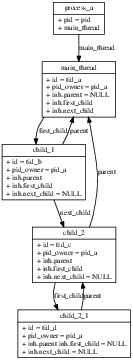
\includegraphics[width=7cm]{gfx/proc-classdiag}
  \caption{Thread tree example.}
  \label{figure:thtree}
\end{figure}

The following notation is used:

\begin{itemize}
  \item \verb+tid_X+ = Thread ID
  \item \verb+pid_a+ = Process ID
  \item \verb+0+ = NULL
\end{itemize}

\verb+process_a+ a has a main thread called \verb+main+. Thread
\verb+main+ has two child thread called \verb+child_1+ and \verb+child_2+.
\verb+child_2+ has created one child thread called \verb+child_2_1+.

\verb+main+ owns all the threads it has created and at the same time child
threads may own their own threads. If parent thread is killed then the
children of the parent are killed first in somewhat reverse order.

\begin{itemize}
  \item \verb+parent+ = Parent thread of the current thread if any
  \item \verb+first_child+ = First child created by the current thread
  \item \verb+next_child+ = Next child in chain of children created by the
        parent thread
\end{itemize}

\section{Examples}

\subparagraph*{process\_a is killed}

Before \verb+process_a+ can be killed \verb+main+ thread must be killed,
because it has child threads its children has to be resolved and killed in
reverse order of creation.

\subparagraph*{child\_2 is killed}

Killing of \verb+child_2+ causes \verb+child_2_1+ to be killed first.


\chapter{Thread Scheduler}

The scheduler in Zeke is conceptually object oriented and all
scheduling entities, CPUs as well as scheduling policies are
implemented as objects in the scheduling system. Each CPU can
be technically populated with a different set of scheduling
policies that are then only executable on that particular
CPU, see figure \ref{figure:objscheds}.

\begin{figure}
  \center
  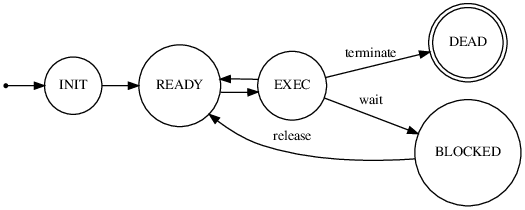
\includegraphics[width=10cm]{gfx/thread-states}
  \caption{Thread states in the scheduler.}
  \label{figure:threadstates}
\end{figure}

\begin{figure}
  \center
  \includegraphics[width=5cm]{proc/objscheds}
  \caption{Scheduler CPU objects for two processor cores and
           per scheduler object scheduling policy objects in
           priority order.}
  \label{figure:objscheds}
\end{figure}
